\documentclass{../../text-style}

\texttitle{Объектно-ориентированное программирование}

\begin{document}

\maketitle
\thispagestyle{empty}

\section{Основные понятия объектно-ориентированного программирования}

Как, наверное, и так известно, в объектно-ориентированном стиле программа представляется в виде набора объектов. \textbf{Объект} --- это набор данных и процедур их обработки, вместе представляющий некую независимую сущность. То есть объект имеет своё состояние и своё поведение, и никто извне объекта не вправе делать предположения о том, как именно он устроен. Объекты общаются друг с другом посредством посылки/приёма сообщений. Важное отличие концепции сообщений от вызова функции --- объект сам решает, как реагировать на сообщение, и тот код, который вызовется как реакция на какое-то сообщение, вообще говоря, заранее (во время компиляции) неизвестен. Кроме того, у объекта есть \textbf{интерфейс} --- собственно, набор сообщений, которые он может обрабатывать. То есть, объект можно представлять себе как чёрный ящик, у которого есть какие-то входы, куда можно послать какие-то данные и получить ответ. В ООП такую точку зрения на объект называют \textbf{инкапсуляцией}, подразумевая под ней одновременно и сокрытие деталей реализации (наружу видно только интерфейс объекта, или набор интерфейсов), и сбор всех данных и методов их обработки в одном месте --- в самом объекте.

Не следует относиться к объектам как к структурам с методами. Объект --- это обособленная часть системы, которая обладает каким-то поведением и взаимодействует с остальным миром через какой-то интерфейс. Пожалуй, самое важное понятие для объектно-ориентированного программирования (как и для программирования вообще и для процесса познания ещё более вообще) --- абстракция. \textbf{Абстракция} --- это выделение существенных характеристик чего-то, что существует в предметной области, чтобы с этим было можно работать. Например, рассмотрим картинку из знаменитой книги Гради Буча <<Объектно-ориентированный анализ и проектирование>>:

\begin{center}
    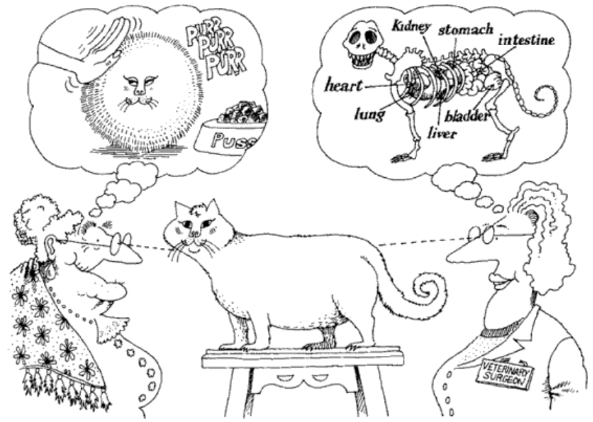
\includegraphics[width=0.5\textwidth]{abstraction.png}
\end{center}

Кот, как объект реального мира, обладает бесконечным количеством различных атрибутов, но интересны нам только некоторые. Причём, какие именно --- зависит от нашей точки зрения. Например, для бабушки важно, что кота можно гладить, а для ветеринара --- что у него есть различные внутренние органы. Кот, как сущность реального мира, может порождать сразу несколько абстракций.

Абстракция хороша тем, что позволяет нам не думать о несущественных деталях. У любой абстракции можно выделить её \textbf{контракты} --- то, что она должна делать, что можно делать с ней и т.д., и её реализацию --- то, как она это должна делать. Инкапсуляция на самом деле разделяет контракты и реализацию объекта, <<пряча>> от пользователя объекта его внутреннюю сложность. Например, тот же кот может быть очень сложно устроен внутри, но бабушка, когда его гладит, имеет право ничего об этом не знать:

\begin{center}
    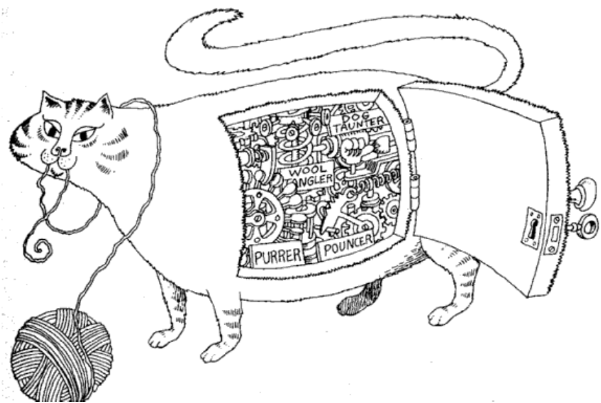
\includegraphics[width=0.5\textwidth]{incapsulation.png}
\end{center}

Ещё одним важным понятием для ООП является \textbf{инвариант} объекта --- некоторый набор условий на состояние объекта, которые выполняются после создания объекта и после вызова каждого его метода всё время жизни объекта. Например, что у квадрата стороны всегда равны, что поле \textit{size} списка должно содержать число, равное количеству элементов списка. Объект сам отвечает за поддержание своего инварианта, и все его методы реализуются в предположении, что инвариант всегда выполняется. Поэтому, в частности, следует избегать публичных полей --- они не контролируются самим объектом, так что инвариант может быть нарушен извне, и объект не сможет этому помешать. Если же поле не является частью инварианта (то есть на него нет никаких условий), это является как правило признаком плохого дизайна --- непонятно, что поле в таком случае делает в этом объекте. Обратите внимание, что инвариант может нарушаться, пока объект находится посреди своего метода (например, когда мы добавляем новый элемент в список, мы могли ещё не успеть обновить \textit{size}). Но при выходе из метода инвариант снова должен начать выполняться.

В некоторых ОО-языках программирования (например, в Java, C++ и C\#) есть понятие класса. \textbf{Класс} --- это тип объекта. Класс описывает, какими полями обладает объект и какие методы у него есть. Типы полей определяет класс, а вот значения полей свои для каждого объекта. Бывают ещё \textbf{поля класса} --- с модификатором \textit{static} в C\#, их значение одинаково для всех объектов данного класса, путать их с полями объекта нельзя. Итак, объект --- экземпляр класса. Например, есть класс <<студент>>, у которого есть такие поля как номер зачётки, оценки за последнюю сессию и т.д., а есть объект <<Иван Иванов>> класса студент, у которого номер зачётки вполне определённый. При этом, скажем, ссылка на закон, согласно которому студенты не идут в армию, не зависит от конкретного студента, поэтому её можно считать полем класса.

Классы могут состоять в отношениях \textbf{генерализации}, то есть между ними может существовать связь <<более общее понятие --- более конкретное понятие>>. Например, всякий студент, я надеюсь, человек. Положим, что у человека есть атрибуты \textit{имя} и \textit{фамилия}, выходит, что и у студента они есть (поскольку любой студент --- человек). В таком случае говорят, что класс <<студент>> является \textbf{наследником} класса <<человек>>, наследует его атрибуты и поведение. Это и есть сущность наследования в ООП --- объект класса-наследника \textbf{является} объектом класса-предка (\textbf{is-a}) и может использоваться везде, где может использоваться объект класса-предка. Зачем это надо --- для переиспользования кода. Мы можем написать функцию/процедуру/метод, который будет работать с объектами наиболее общего типа, для которого этот код имеет смысл, а обрабатываться будут на самом деле объекты более узких типов, которые могут быть практически полезны. Например, сортировке пузырьком плевать, что сортировать, лишь бы это что-то умело сравнивать себя с другим таким же чем-то. Сортировку пузырьком можно написать над объектами класса <<штука, которая имеет метод сравнения>>, и она будет работать, даже не зная, что именно она сортирует --- числа или столбцы матрицы. Ещё переиспользования кода можно добиться, определяя общие атрибуты и методы двух классов в одном общем классе-предке. Например, отчислить можно и студентов и аспирантов, так что вместо того, чтобы описывать, как именно отчислять студентов и аспирантов, можно описать, как надо отчислять объект класса <<учащийся>>, классы <<студент>> и <<аспирант>> наследуют метод отчисления автоматически. 

Кстати, такого рода переиспользование кода и переиспользование кода предыдущего вида вообще говоря независимы. То, что использует свойства отношения <<является>>, называется в науке о системах типов <<сабтайпингом>> (или subtype polymorphism, полиморфизмом подтипов) и является довольно важным понятием, на которое завязаны системы типов современных ОО-языков, второе никакого отношения к типам вообще не имеет (напомним, что тип --- это набор значений и допустимых операций над ними, как именно реализованы операции и что они делают, систему типов языка не интересует --- что реализация описана в предке или в потомке, систему типов не интересует тем более, она проверяет лишь корректность применения операций). В С++ эти два вида наследования явно разделены, во всех нормальных языках наследование влечёт сабтайпинг.

Тут уже должно быть понятно, что один объект может иметь несколько типов сразу --- являться экземпляром нескольких классов. Иван Иванов --- экземпляр класса <<студент>> и экземпляр класса <<человек>>, и вообще, экземпляр некоего класса является и экземпляром всех классов-предков. Более того, объект может являться экземпляром нескольких несвязанных классов --- например, тот же гипотетический Иван может являться экземпляром класса <<студент>> и экземпляром класса <<любитель дотки>>. В таком случае объект имеет все атрибуты и первого, и второго класса. Более того, объекты могут вообще менять свои классы во время жизни --- например, когда наш Иван закончит университет, он перестанет быть студентом, но не перестанет быть Иваном, то есть не лишится своей идентичности. Такие дела огорчают статическую типизацию, поэтому в распространённых языках не используются. Более того, в нормальных языках объект всегда создаётся как экземпляр некоего известного во время компиляции класса, так что чтобы у нас был объект Иван, нам потребуется сначала класс <<студент --- любитель дотки>>, который будет наследовать от классов <<студент>> и <<любитель дотки>>, зато потом можно создать кучу студентов --- любителей дотки. Важно понимать, что каждый класс, экземпляром которого является объект, задаёт интерфейс доступа к этому объекту --- к Ивану можно обратиться как к студенту (например, поставить ему зачёт), или как к любителю дотки (например, поговорить с ним о последней катке). Объект будет один и тот же, а вот набор допустимых действий с ним и его поведение могут быть разными. Это же касается классов и в иерархии наследования --- интерфейс, по которому можно обратиться к объекту как к экземпляру класса-предка, уже, чем интерфейс объекта как экземпляра класса-потомка.

В нормальных языках (со строгой статической типизацией, как C++, Java и C\#) из всего множества типов, которым соответствует объект, выделяется один --- тот, с которым этот объект создавался. Этот тип имеет физический смысл <<настоящего>> типа объекта, того, <<чем является объект на самом деле>>. Конечно, объект на самом деле является объектом любого из типов-предков, но как он реализует свои операции --- написано именно в его <<настоящем>> типе. До реализации операций, как уже говорилось, системе типов дела нет, так что с точки зрения теории всё хорошо, а с точки зрения практики это понятие весьма важно для полиморфных вызовов. Но про это чуть потом, пока надо запомнить, что этот <<настоящий>> тип объекта называется его \textbf{типом времени выполнения} (\textbf{runtime type}), а типы объекта, про которые знает компилятор, и операциями которых можно пользоваться в программе --- \textbf{типами времени компиляции} (\textbf{compile-time type}). Разницу можно пояснить на таком примере:

\begin{minted}{csharp}
Shape a = new Circle();
\end{minted}

У переменной \textit{a} будет тип времени компиляции \textit{Shape} (и все его предки, да), и вызывать методы мы можем только те, которые объявлены в \textit{Shape} (или его предках, да). А тип времени выполнения у этой же переменной будет \textit{Circle}, но компилятор про это не знает (знает, но забудет строчкой ниже, поскольку переменная объявлена как \textit{Shape}), и, в силу строгой типизированности C\#, вызывать методы, специфичные для \textit{Circle}, у переменной \textit{a} будет нельзя. Для тех, кто не в теме --- не надо пугаться, про это ещё будет ниже.

Ещё одним важным для ООП принципом является то, что потомки могут переопределять поведение предков. Например, обычно если людям рассказывать про ООП, им плевать, а если студентам рассказывать про ООП, они получают некие знания. Заметьте, что человеку можно рассказывать про ООП, следовательно, и студенту тоже, и преподу по сути всё равно, кому рассказывать, главное, чтобы рассказывать было можно --- но результат получается разный. Собственно, в этом и состоит большая часть радости от наследования, и возможность переопределения поведения + сабтайпинг обычно и называют \textbf{полиморфизмом}. Объект, как говорилось, реагирует на сообщение, сообщение может быть послано объекту как экземпляру класса-родителя, а как оно будет обработано --- решает сам объект, это зависит от его <<настоящего>> типа. Зачем это нужно --- опять-таки, для переиспользования кода, когда в базовом классе определяется некоторое поведение по умолчанию, а в некоторых классах-потомках это поведение переопределяется, или для того, чтобы можно было менять поведение некоего кода прямо во время выполнения. Например, у нас есть код, выводящий матрицу по спирали. Мы хотим в зависимости от желания пользователя вывести результат в файл или на консоль. Ему можно передать объект класса <<Выводилка>>, у которого есть метод <<вывести>>, который, скажем, просто никуда ничего не выводит, от него унаследованы два класса <<ВыводилкаНаКонсоль>> и <<ВыводилкаВФайл>>, в которых метод <<вывести>> переопределён соответственно. Метод печати матрицы по спирали получает в качестве параметра объект типа <<Выводилка>> и вызывает его метод <<вывести>>. А основная программа в зависимости от выбора пользователя создаёт объект либо одного класса, либо другого --- и передаёт параметром печаталке спирали. Очень удобно, печаталка даже не знает, что и куда она там выводит.

Или ещё один пример: рассмотрим графический редактор с разными геометрическими фигурами. Можно описать такую иерархию наследования:

\begin{center}
    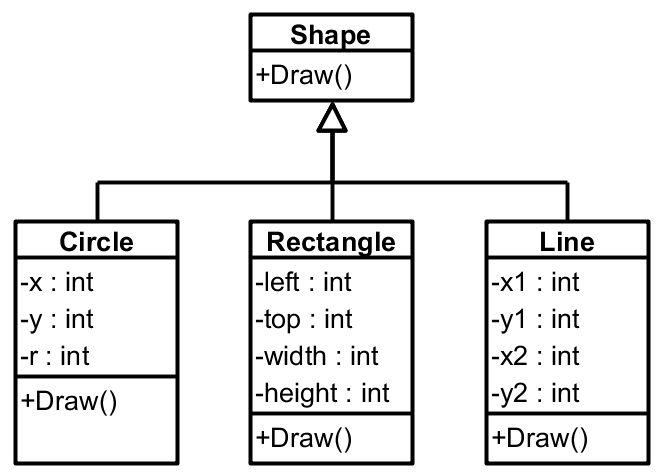
\includegraphics[width=0.5\textwidth]{polymorphism.png}
\end{center}

Класс \textit{Shape} определяет операцию \textit{Draw}, которую должны реализовать все его потомки, от него наследуются круг, прямоугольник и линия, каждый из которых реализует \textit{Draw} по-разному. И тогда мы можем нарисовать все фигуры на сцене, просто один раз пройдя по списку объектов класса \textit{Shape} --- поскольку у нас есть полиморфизм, каждый из этих объектов на самом деле будет какой-то конкретной фигурой, которая реализует метод \textit{Draw} по-своему. И каждая фигура отрисует себя так, как она должна себя рисовать, при этом наш код даже не будет знать, что это была за фигура (более того, конкретный класс-фигура может ещё не существовать в тот момент, когда мы пишем код редактора --- например, взяли и добавили стрелочки и звёзды). Вот небольшой пример кода, поясняющий сказанное:

\begin{minted}{csharp}
List<Shape> shapes = new List { new Circle(0, 0, 5), new Line(0, 0, 10, 10) };

foreach (var shape in shapes)
{
    shape.Draw();
}
\end{minted}

Для того, чтобы не придумывать реализацию по умолчанию для методов, которые бессмысленны в родительском классе --- типа нашего метода \textit{Draw} для абстрактной фигуры \textit{Shape}, придумали понятие абстрактного метода --- метода, для которого реализация не определена вовсе. Мы объявляем, что класс имеет такой-то метод с таким-то набором параметров и таким-то возвращаемым значением, но как он реализован --- определяют классы-потомки. Понятно, что объект класса с абстрактным методом создать нельзя --- он не будет знать, что делать, если абстрактный метод вызовут. А вот если объект имеет <<настоящий>> тип класс-потомок, у него этот метод переопределён, так что вызвать его можно и существование объекта осмысленно. Классы с абстрактными методами называются абстрактными классами. Есть ещё интерфейсы --- это по сути классы, у которых все методы абстрактные. Надо понимать их так --- они определяют некий интерфейс, или протокол взаимодействия, которому удовлетворяет объект, его реализующий, и всё, без каких-либо попыток предоставить реализацию. Тогда \textit{Shape} можно сделать интерфейсом, а конкретные фигуры --- классы, его реализующие. Код можно писать в терминах интерфейсов, подставляя на их место объекты конкретных классов уже во время выполнения, это повышает уровень абстрактности кода, а значит, и возможностей для его переиспользования.

\section{Объектно-ориентированное программирование в C\#}

\subsection{Ссылочные типы и типы-значения}

Если объекты-потомки можно использовать везде, где используются объекты-предки, то их, например, и в массивы можно класть, и копировать. А если они разные по размеру, что делать? Индексация в массивах выполняется путём умножения индекса на размер элемента, так что просто хранить в массиве разные по размеру элементы нельзя. Надо использовать не сами объекты, а указатели. Указателей в C\# нет (ну, почти), вместо них используются ссылки. Ссылки в C\# почти такие же, как в С++, если кто в курсе, только в С++ если ссылке присвоили значение, то поменять его уже нельзя, только значение объекта, на который она ссылается. В C\# (как и в Java, кстати) присваивание ссылочной переменной --- это именно присваивание ссылочной переменной, а не объекту, на который она ссылается, в этом смысле ссылочные переменные больше похожи на указатели в C. Если у нас есть такой вот код:

\begin{minted}{csharp}
var circle1 = new Circle(0, 0, 5);
var circle2 = new Circle(10, 10, 15);
var circle3 = null;

circle3 = circle2;
\end{minted}

то на картинке это выглядит как-то так:

\begin{center}
    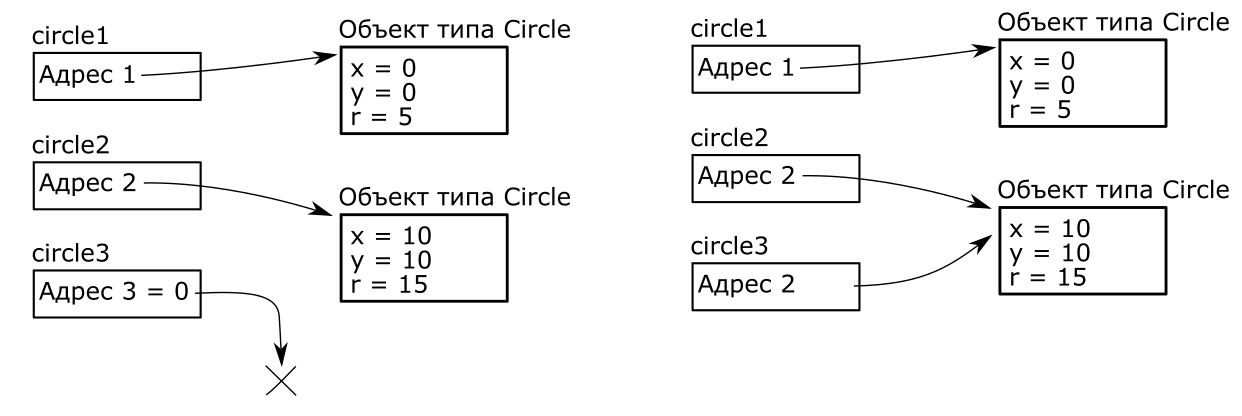
\includegraphics[width=\textwidth]{referenceTypes.png}
\end{center}

Очень похоже на указатель в С, только доступа к содержимому самой ссылочной переменной у нас нет. Например, арифметика указателей не получится в принципе, сделать ссылку на ссылку тоже нельзя. Зато и разыменовывать такой <<указатель>> не нужно: можно писать просто \textit{circle3.x}. Важно только помнить, что <<=>> не вызывает оператор присваивания класса \textit{Circle}, а присваивает значение ссылочной переменной, а <<==>> не сравнивает значения объектов, а проверяет, что две ссылочные переменные ссылаются на один объект (если операторы не перегружены, по умолчанию поведение именно такое).

Для ссылочных переменных нет никакого специального синтаксиса объявления, просто все переменные ссылочных типов --- ссылочные. Вообще все типы делятся в C\# на типы-значения и ссылочные типы (в Java, кстати, тоже). Разница между ними в выделении памяти и в понятии \textbf{идентичности} (\textbf{identity}) (и связанных с ним заморочек, касающихся поведения операторов копирования и сравнения). Начнём с памяти. Под ссылочные типы память выделяется всегда в куче (под то, на что указывают ссылки, а не под сами ссылки, это важно понимать), всегда с использованием оператора \textit{new}. Это в C мы могли выбирать, на стеке заводить объект или в куче (\textit{Point *a = malloc(sizeof(Point));} или просто \textit{Point a;}), в C\# всё решили за нас. Под типы-значения память выделяется всегда на стеке, соответственно, время жизни объекта-значения --- пока он не вышел из области видимости. Это удобно, потому что избавляет нас от необходимости думать, когда же наш объект умрёт (хотя тут это не так важно, как в С, потому что в куче работает сборщик мусора, и <<забытые>> объекты всё равно не проживут долго).

Идентичность некоторым образом связана с выделением памяти. Идентичность ссылочных типов данных определяется их местоположением в куче (просто адресом объекта), так что две ссылки равны, если они указывают на один и тот же объект. Это важно. Если у нас есть два абсолютно одинаковых объекта, с абсолютно одинаковыми полями, то это всё равно будут разные объекты. Например, бывают однофамильцы, бывают люди, у которых совпадает имя и фамилия, и это всё равно разные люди. С типами-значениями всё не так, их идентичность определяется их значением. Два числа <<1>> равны, глубоко всё равно, что это за единицы и где они физически находятся. То же относится к, скажем, точкам на плоскости --- две точки равны, если их координаты совпадают.

Так вот, ссылочные типы --- это классы (в том числе, строки, массивы, исключения, делегаты). Типы-значения --- это примитивные типы (\textit{int}, \textit{bool}, \textit{double} и т.д.), типы-перечисления и структуры. Некоторая тонкость заключается в том, что формально в C\# всё является классом (и наследуется от общего базового класса Object, но об этом потом), ведь даже у примитивных типов есть методы (\textit{1.ToString()} прекрасно будет работать, например), но некоторые классы наследуют от класса \textit{ValueType}, вот они-то и будут типами-значениями. К счастью, в отличие от той же Java, в C\# есть перегрузка операторов, поэтому со ссылочными типами не так неудобно работать, как в той же Java --- сравнивать строки (ссылочные типы!) оператором <<==>> в C\# можно, и это приведёт к ожидаемым результатам (в Java можно было сравнить две одинаковые строки и получить, что они не равны, просто потому, что они лежат по разным адресам в памяти, впрочем, в C с \textit{char*} было так же; в C\# всё будет ок, они будут равны). Для ссылочных типов ещё определено понятие ссылки, которая указывает в никуда --- \textit{null} (как в С \textit{NULL}).

Со ссылочными типами связана ещё одна неприятная тонкость. Рассмотрим подпрограмму, которая должна бы возвращать с помощью переменной \textit{s3} сумму строк, хранящихся в переменных \textit{s1} и \textit{s2}:

\begin{minted}{csharp}
static void Add(string s1, string s2, string s3)
{
    s3 = s1 + s2;
}
\end{minted}

На первый взгляд кажется, что работать не должно --- мы меняем значение параметра функции, так что извне этого изменения видно быть не должно. Но потом мы принимаем во внимание, что строки --- ссылочные типы, так что передаются не сами строки, а ссылки на строки, так что если мы что-то с этими строками делаем, то извне это должно быть видно. В С++, например, значение \textit{s3} вовне бы благополучно поменялось, если бы он передавался как ссылка, с амперсандом. Но потом мы понимаем, что объекты-то передаются по ссылке, но ссылочные переменные передаются по значению, то есть если строку поменять, она честно поменяется, но если ссылочной переменной \textit{s3} присвоить новую строку (результат сложения), то она просто забудет про старую строку, начнёт указывать на новую, и помрёт при выходе из метода (к этому моменту те, кто не в теме, должны уже запутаться, но на всякий случай скажу, что тут-то и проявляется отличие семантики ссылок от C++ --- в C++ ссылки немутабельны, начав указывать на какой-то объект, ссылка в С++ указывает на него всегда, а в C\# и Java ссылки мутабельны, то есть могут менять объект, на который они указывают). В данном случае, конечно, лучше возвращать результат конкатенации, и вызывающий уже может делать с ним, что хочет, но в отличие от Java, где надо делать только так, и, например, функцию \textit{swap} никогда не написать, в C\# есть ключевые слова \textit{ref} и \textit{out}, которые работают как настоящая передача параметров по ссылке в C++. Передача ссылочных переменных по ссылке, так-то. Выглядит это так:

\begin{minted}{csharp}
static void Add(string s1, string s2, ref string s3)
{
    s3 = s1 + s2;
}

private static void Main(string[] args)
{
    string s1 = "a";
    string s2 = "b";
    string s3 = "c";
    Add(s1, s2, ref s3);
}
\end{minted}

Или то же самое с \textit{out}:

\begin{minted}{csharp}
static void Add(string s1, string s2, out string s3)
{
    s3 = s1 + s2;
}

private static void Main(string[] args)
{
    string s1 = "a";
    string s2 = "b";
    Add(s1, s2, out string s3);
}
\end{minted}

С типами-значениями \textit{ref} и \textit{out}, естественно, тоже работают, и эффект от этого вполне ожидаем. На этом про ссылочные типы пока всё, к конструкциям типа \textit{listElement.next = listElement.next.next;} вполне можно привыкнуть, если делать домашку.

\subsection{Конструкторы}

Объекты создаются с помощью конструкторов, и только с помощью конструкторов. Конструктор --- это такой специальный метод, который не имеет типа возвращаемого значения (вообще, даже \textit{void}), и называется так же, как и класс. Конструктор в классе можно не писать, тогда для него будет определён конструктор по умолчанию, который не принимает аргументов и ничего не делает. Зачем они нужны и как их вызывать: когда мы пишем, например, \mintinline{csharp}|Circle circle = new Circle(0, 0, 10);|, то во-первых, под объект класса \textit{Circle} выделяется память на куче, достаточная для хранения всех его полей (включая поля классов-предков), во-вторых, вызывается его конструктор, который должен инициализировать его поля какими-то осмысленными значениями и сделать всё, что нужно, чтобы класс можно было использовать по назначению (ну, не всё так просто, потому что есть ещё поля классов-предков, для инициализации которых используются конструкторы предков, которые вызываются перед нашим конструктором, так что конструирование объекта начинается с вызова конструкторов вверх по цепочке наследования, а затем исполнения конструкторов вниз, до конструируемого объекта, но можно пока не грузиться). В конструкторе можно писать любой код, например, открытие сетевого соединения, чтение из файла, и т.д. Заканчиваться исполнение конструктора должно тем, что для объекта выполнен его инвариант (вспомните, я в начале пары говорил), и объект готов обрабатывать запросы. То есть, если сначала надо создать объект (при этом вызовется конструктор), а потом вызвать какой-нибудь метод вроде \textit{Init} (или, ещё ужаснее, вручную заполнять поля или свойства), то кто-нибудь когда-нибудь наверняка забудет это сделать, и всё сломается. Конструктор же забыть вызвать не получится, иных способов создать объект нет, так что всю инициализацию, если это возможно, надо делать там.

Реализован конструктор может быть, например, так:

\begin{minted}{csharp}
class Circle
{
    public Circle(int x, int y, int r)
    {
        this.x = x;
        this.y = y;
        this.r = r;
    }

    private int x;
    private int y;
    private int r;
}
\end{minted}

Никакой магии, кроме, пожалуй, использования ключевого слова \textit{this} --- ссылки на текущий объект. Этой штукой тут надо пользоваться, поскольку имена параметров конструктора перекрывают поля класса, и если бы мы просто написали \textit{x = x;}, то ничего бы не произошло. \textit{this} же указывает на тот объект, у которого был вызван метод, так что \textit{this.x} вернёт нам значение поля \textit{x} того экземпляра класса \textit{Circle}, с которым мы сейчас работаем. Вообще, поля в методах доступны и непосредственно, писать всюду \textit{this} не нужно (хотя и считается хорошим тоном, да). Кстати, все поля классов в C\# всегда инициализируются значениями по умолчанию (\textit{0} для целых, \textit{false} для булевых, \textit{null} для всех ссылочных типов и т.д., кстати, строки по умолчанию будут не пустыми, а \textit{null}). Конструкторы можно перегружать, то есть определять в классе несколько конструкторов с разными параметрами, и даже вызывать из одного другой, например, так:

\begin{minted}{csharp}
class Circle
{
    public Circle(int x, int y, int r)
    {
        this.x = x;
        this.y = y;
        this.r = r;
    }

    public Circle(int r)
        : this(0, 0, r)
    {
    }

    private int x;
    private int y;
    private int r;
}
\end{minted}

Тут \textit{this} имеет несколько другое значение, но суть та же --- тот объект, от которого мы вызываем метод. Можно вызывать конструктор предка с помощью ключевого слова \textit{base}, так же, как и \textit{this}. Если объявлен хоть один конструктор, конструктор по умолчанию не генерируется, но его несложно при желании реализовать руками: 

\begin{minted}{csharp}
Circle()
{
}
\end{minted}

Порядок вызовов при создании объекта некого класса (будем называть его дочерним классом) такой.
\begin{itemize}
    \item Создается объект, в котором все поля данных имеют значения по умолчанию (нули на двоичном уровне представления).
    \item Вызывается конструктор дочернего класса.
    \item Конструктор дочернего класса вызывает конструктор родителя (непосредственного прародителя), а также по цепочке все прародительские конструкторы и инициализации полей, заданных в этих классах, вплоть до класса \textit{Object}.
    \item Проводится инициализация полей родительской части объекта значениями, заданными в декларации родительского класса.
    \item Выполняется тело конструктора родительского класса.
    \item Проводится инициализация полей дочерней части объекта значениями, заданными в декларации дочернего класса.
    \item Выполняется тело конструктора дочернего класса.
\end{itemize}

\subsection{Наследование}

Наследование тут описывается очень просто, через двоеточие указывается класс-предок:

\begin{minted}{csharp}
class Shape
{
    public Shape() 
    {
    }

    public Shape(int x, int y)
    {
        this.x = x;
        this.y = y;
    }

    protected int x;
    protected int y;
}

class Circle : Shape
{
    Circle(int x, int y, int r)
    {
        this.x = x;
        this.y = y;
        this.r = r;
    }

    Circle(int r)
        : base(0, 0)
    {
    }

    private int r;
}
\end{minted}

Заодно можно видеть использование ключевого слова \textit{base} для вызова конструктора предка (если нет, то вызывается конструктор предка по умолчанию, тот, что без параметров, если он есть, иначе ошибка компиляции), и ключевое слово \textit{protected}, означающее, как и следует ожидать, то, что поле/метод будут видны только потомкам. Наследоваться можно только от одного класса, множественного наследования нет. Почему --- множественное наследование создаёт некие трудности само по себе. Например, ситуация, называемая ромбовидным наследованием: есть класс \textit{A}, в котором объявлен метод \textit{a}, классы \textit{B} и \textit{C}, которые переопределяют метод \textit{a}, причём каждый по-разному, и класс \textit{D}, который наследует от \textit{B} и от \textit{C} --- какую из реализаций метода a он получит? В С++ множественное наследование разрешено, в более современных языках --- нет. Зато класс может реализовывать несколько интерфейсов.

\subsection{Интерфейсы, абстрактные классы}

Интерфейс описывается вот так:

\begin{minted}{csharp}
interface IDrawable
{
    void Draw();
}
\end{minted}

И реализуется вот так:

\begin{minted}{csharp}
class Shape : IDrawable
{
    public Shape() 
    { 
    }

    void Draw()
    {
        Console.Write("Drawing Shape");
    }

    protected int x;
    protected int y;
}
\end{minted}

Можно унаследоваться от одного класса и скольки угодно интерфейсов одновременно. Почему --- интерфейс всего лишь декларирует методы, которые должны быть у реализующих его объектов, как объект их реализует --- его дело. Собственно, если есть два интерфейса с методами с одинаковыми именами и набором параметров, то они оба могут быть реализованы одним методом, и всё будет ок, так что никакого ромбовидного наследования тут не возникает. Все методы в интерфейсе не могут иметь реализацию, то есть являются абстрактными. Кстати, при реализации интерфейса можно явно указать, метод какого именно интерфейса мы реализуем, как раз если есть два интерфейса с одинаковыми методами и мы хотим сделать две разные реализации:

\begin{minted}{csharp}
class Shape : IDrawable
{
    public Shape() 
    { 
    }

    void IDrawable.Draw()
    {
        Console.Write("Drawing Shape");
    }

    protected int x;
    protected int y;
}
\end{minted}

Теперь метод \textit{Draw()} нельзя вызывать просто от объекта, надо сначала привести его к тому интерфейсу, чей \textit{Draw()} мы реализовали (иначе как компилятор узнает, какой из \textit{Draw()} мы имеем в виду, если их много?):

\begin{minted}{csharp}
var shape = new Shape();
((IDrawable)shape).Draw();
\end{minted}

Обычному классу тоже можно сделать абстрактный метод (например, не знаем мы, как рисовать просто фигуру, могли бы сделать у \textit{Shape} метод \textit{Draw} абстрактным), для этого перед методом надо написать ключевое слово \textit{abstract}. Абстрактные методы обязаны быть реализованы во всех неабстрактных потомках, то есть, например, \textit{Circle} обязан реализовать \textit{Draw}, либо же оставить его абстрактным, чтобы его реализовали потомки \textit{Circle}. Класс, у которого есть хоть один абстрактный метод, сам абстрактный, и должен быть помечен ключевым словом \textit{abstract}, так:

\begin{minted}{csharp}
abstract class Shape
{
    public Shape() 
    { 
    }

    public abstract void Draw();

    protected int x;
    protected int y;
}
\end{minted}

Объекты абстрактных классов создавать, естественно, нельзя, иначе в момент вызова абстрактного метода у объекта такого класса наступит печаль и непонимание, что ему делать. Тем не менее, конструкторы в абстрактных классах --- это вполне ок, поскольку они будут вызываться при конструировании потомков.

\subsection{Полиморфизм}

Польза от абстрактных классов, интерфейсов, да и наследования вообще проявляется при использовании полиморфных вызовов. Как уже говорилось, полиморфизм позволяет в классах-потомках переопределять поведение классов-предков. В C\# это делается так: если мы хотим, чтобы метод можно было переопределить, мы помечаем его ключевым словом \textit{virtual}, в потомке, в котором мы его хотим переопределить, объявляем метод с точно такой же сигнатурой (именем и набором параметров), и помечаем его ключевым словом \textit{override}. Пример:

\begin{minted}{csharp}
class Shape
{
    public virtual void Draw()
    {
        Console.WriteLine($"Drawing Shape with coords ({x}, {y})");
    }

    protected int x;
    protected int y;
}

class Circle : Shape
{
    public Circle(int x, int y, int r)
    {
        this.x = x;
        this.y = y;
        this.r = r;
    }

    public override void Draw()
    {
        Console.WriteLine($"Drawing Circle with radius {r}");
    }

    private int r;
}

class Rectangle : Shape
{
    public Rectangle(int x, int y, int width, int height)
    {
        this.x = x;
        this.y = y;
        this.width = width;
        this.height = height;
    }

    public override void Draw()
    {
        base.Draw();
        Console.WriteLine($"Drawing Rectangle with width={width} and height={height}");
    }

    protected int width;
    protected int height;
}
\end{minted}

Тут ещё можно видеть использование ключевого слова \textit{base} для вызова метода предка в переопределённом методе у потомка. Теперь пример того, как этими виртуальными методами пользоваться (собственно, магия полиморфизма):

\begin{minted}{csharp}
private static void Main(string[] args)
{
    var circle = new Circle(0, 0, 10);
    var rectangle = new Rectangle(0, 0, 10, 10);
    var list = new System.Collections.Generic.List<Shape>();
    list.Add(circle);
    list.Add(rectangle);

    foreach (var shape in list)
    {
        shape.Draw();
    }
}
\end{minted}

Деталями использования генерика-списка можно пока не грузиться, суть в том, что мы побросали в список шейпов разные фигуры, а потом просто прошлись и отрисовали их все, не заморачиваясь их типом времени исполнения. Поскольку все фигуры наследуют от \textit{Shape}, то у них у всех всё равно должен быть метод \textit{Draw}, так что его можно вызвать, имея ссылку с типом времени компиляции \textit{Shape}. Обратите внимание, что если мы добавим ещё фигур в нашу иерархию, то код отрисовки менять будет вообще не надо! В этом и есть основное преимущество при использовании объектно-ориентированного подхода, мы можем создавать каркасы приложений, которые расширяются с помощью классов-наследников, тогда сам каркас трогать не надо (он может нам поставляться даже без исходников), а мы просто дописываем немного кода, и всё работает. Именно так устроены средства разработки пользовательских интерфейсов в объектно-ориентированных языках.

Что получится:

\begin{minted}{text}
Drawing Circle with radius 10
Drawing Shape with coords (0, 0)
Drawing Rectangle with width=10 and height=10
Для продолжения нажмите любую клавишу . . .
\end{minted}

То же самое касается абстрактных методов:

\begin{minted}{csharp}
abstract class Shape
{
    public abstract void Draw();

    protected int x;
    protected int y;
}

class Circle : Shape
{
    public Circle(int x, int y, int r)
    {
        this.x = x;
        this.y = y;
        this.r = r;
    }

    public override void Draw()
    {
        Console.WriteLine($"Drawing Circle with radius {r}");
    }

    private int r;
}
\end{minted}

Если \textit{override} не написать, то компилятор выдаст предупреждение --- вы действительно объявляете новый метод или пытаетесь переопределить метод класса предка? Если хотите именно новый, это надо явно сказать с помощью немного неоригинального ключевого слова new:

\begin{minted}{csharp}
class Shape
{
    public virtual void Draw()
    {
        Console.WriteLine($"Drawing Shape with coords ({x}, {y})");
    }

    protected int x;
    protected int y;
}

class Circle : Shape
{
    public Circle(int x, int y, int r)
    {
        this.x = x;
        this.y = y;
        this.r = r;
    }

    public new void Draw()
    {
        Console.WriteLine($"Drawing Circle with radius {r}");
    }

    private int r;
}
\end{minted}

В чём разница с \textit{override}: при полиморфном вызове вызовется метод предка (ну, типа потомок его не переопределяет, \textit{Circle.Draw} --- это другой метод, не имеющий отношения к \textit{Shape.Draw}). 

Ещё есть ключевое слово \textit{sealed}, говорящее, что метод нельзя дальше переопределять, или, если оно применено к классу, от класса нельзя наследоваться. Это используется в системных библиотеках, чтобы, например, злоумышленники не унаследовались от строки и не вставили туда код, отправляющий пароли на сервер, после чего подсунули такие строки вместо обычных строк в пользовательскую программу. У вас таких проблем пока быть не должно, так что не буду подробно.

\subsection{Модификаторы}

Помимо \textit{new} и \textit{sealed} у методов, полей и самих классов могут быть модификаторы видимости. Видимость определяет, откуда можно использовать класс, его метод или поле. Модификаторы видимости в C\# такие:

\begin{itemize}
    \item \mintinline{csharp}|public| --- применяется к типам и членам (то есть полям, методам, свойствам, событиям), доступ без ограничений;
    \item \mintinline{csharp}|protected| --- применяется только к членам, доступ в типе и его потомках;
    \item \mintinline{csharp}|internal| --- применяется к типам и членам, доступ только внутри сборки (то есть одного проекта, который собирается в одну .dll-ку или .exe-файл);
    \item \mintinline{csharp}|protected internal| --- применяется к типам и членам, доступ внутри сборки \textbf{или} в потомках;
    \item \mintinline{csharp}|private| --- применяется к типам и членам, доступ только внутри типа;
    \item по умолчанию для типов \mintinline{csharp}|internal|, для членов --- \mintinline{csharp}|private|.
\end{itemize}

Бывает ещё модификатор \textit{partial}, который применяется к классам и говорит компилятору, что в этом файле есть только часть описания класса, и может быть ещё один или несколько файлов, определяющих другие члены класса. Используется это в основном для того, чтобы один класс мог содержать рукописные и автоматически сгенерированные части и чтобы при перегенерации рукописный код не затирался (например, так работает дизайнер пользовательских интерфейсов). Использовать \textit{partial} для логической группировки полей и методов --- плохая идея, если возникла такая потребность, вам, скорее всего, нужно просто несколько разных классов.

\subsection{Вложенные классы}

Классы могут содержать внутри себя описания типов, в частности, других классов (уровней такой вложенности может быть много). Например,

\begin{minted}{csharp}
class Circle
{
    private readonly Point pos;
    private readonly int r;

    private class Point
    {
        public int x;
        public int y;
    }

    public Circle(int x, int y, int r)
    {
        pos = new Point {x = 10, y = 10};
        this.r = r;
    }

    public void Draw() =>
        Console.WriteLine($"({pos.x}, {pos.y}), radius {r}");
}
\end{minted}

Тут класс \textit{Point} объявлен внутри класса \textit{Circle} как \textit{private} вложенный класс, поэтому доступен он только внутри класса \textit{Circle} (где и используется как тип одного из полей). Полезно для обеспечения инкапсуляции.

\subsection{Приведение типов}

Есть ещё явное и неявное приведение типов. От потомка к предку преобразование возможно всегда (потому что потомок и так является предком, да), так что выполняется автоматически. От предка к потомку каст (преобразование, от англ. cast) не всегда возможен: если \textit{Circle} всегда \textit{Shape}, то \textit{Shape} может оказаться либо \textit{Circle}, либо \textit{Rectangle}. Однако если мы уверены относительно типа времени выполнения, мы можем сделать явный каст вручную: 

\begin{minted}{csharp}
Shape shape = new Circle();
Circle circle = (Circle)shape;
\end{minted}

Если мы неправы, программа упадёт с исключением. Есть оператор \textit{as}, который делает то же самое, но в случае неудачи тихо возвращает \textit{null}:

\begin{minted}{csharp}
Shape shape = new Circle();
Circle circle = shape as Circle;
\end{minted}

Есть ещё оператор проверки типа времени выполнения \textit{is}:

\begin{minted}{csharp}
Shape shape = new Circle();
if (shape is Circle) 
{
    Circle circle = (Circle)shape;
}
\end{minted}

Или даже так, сразу же с объявлением переменной приведённого типа:

\begin{minted}{csharp}
Shape shape = new Circle();
if (shape is Circle circle) 
{
    ...
}
\end{minted}

Эту же конструкцию можно использовать внутри \textit{switch}, чтобы делать что-нибудь в зависимости от типа переменной:

\begin{minted}{csharp}
switch (shape)
{
    case Circle c:
        WriteLine($"circle with radius {c.Radius}");
        break;
    case Rectangle s when (s.Length == s.Height):
        WriteLine($"{s.Length} x {s.Height} square");
        break;
    case Rectangle r:
        WriteLine($"{r.Length} x {r.Height} rectangle");
        break;
    default:
        WriteLine("<unknown shape>");
        break;
    case null:
        throw new ArgumentNullException(nameof(shape));
}
\end{minted}

Каст от предка к потомку называется понижающим кастом, каст от потомка к предку называется повышающим кастом. Использование понижающих кастов свидетельствует о непродуманной архитектуре системы --- если мы точно знаем тип времени выполнения переменной, то почему бы не сделать его типом времени компиляции? Однако же, в совокупности с оператором \textit{is} он бывает весьма полезен, и всё-таки используется в промышленном коде.

\subsection{System.Object}

Корнем иерархии наследования в C\# является класс \textit{System.Object}. От него наследуются все типы в языке вообще, не только классы. Вот иерархия наследования основных типов в C\#:

\begin{center}
    \begin{scriptsize}
        \begin{forest}
            for tree={rectangle,draw,l sep=1cm,s sep=5mm,edge=open triangle 60-}
            [Object
                [ValueType
                    [Enum]
                    [Элементарные типы]
                    [Пользовательские структуры]
                ]
                [Array]
                [Delegate]
                [Exception]
                [Пользовательские классы]
                [...]
            ]
        \end{forest}
    \end{scriptsize}
\end{center}

Тип \textit{ValueType} имеет специальное значение для компилятора --- все его наследники считаются типами-значениями. Впрочем, отнаследоваться от него вручную не получится, это ошибка компиляции. Фактически, наследование от него --- это объявление своей структуры. От \textit{ValueType} же наследуются все enum-ы и все элементарные типы (\textit{int}, \textit{double}, \textit{bool} и т.д.). Все пользовательские классы напрямую или опосредованно наследуются от \textit{System.Object}.

В самом \textit{System.Object} определено всего шесть методов и два \textit{private}-поля. Методы такие:

\begin{itemize}
    \item \textit{Equals} --- виртуальный метод, предназначенный для сравнения объектов; напомню, что оператор <<==>> по умолчанию сравнивает адреса объектов в памяти, Equals как раз нужен для того, чтобы можно было сравнивать объекты по значениям их полей;
    \item \textit{GetHashCode} --- виртуальный метод, возвращающий хеш-значение для объекта в виде целого числа (любого), реализация по умолчанию возвращает просто адрес объекта для ссылочных типов и значение для типов-значений;
    \item \textit{ToString} --- виртуальный метод, который должен возвращать строковое представление объекта, для удобства отладки и логирования;
    \item \textit{GetType} --- невиртуальный метод, возвращающий объект-тип объекта, нужен для рефлексии;
    \item \textit{MemberwiseClone} --- невиртуальный защищённый метод, создающий копию объекта путём копирования всех его полей, нужен для сериализации/десериализации;
    \begin{itemize}
        \item обратите внимание, этот метод создаёт объект, не вызывая конструктор;
    \end{itemize}
    \item \textit{Finalize} --- виртуальный защищённый метод, говорящий, что делать, когда объект собирается удалить сборщик мусора.
\end{itemize}

В памяти каждый объект представляется следующим образом. Положим, у нас есть код

\begin{minted}{csharp}
void Example() 
{
    Employee e = 
        new Manager();
    e.GenProgressReport();
}
\end{minted}

Тогда в памяти всё будет выглядеть так:

\begin{center}
    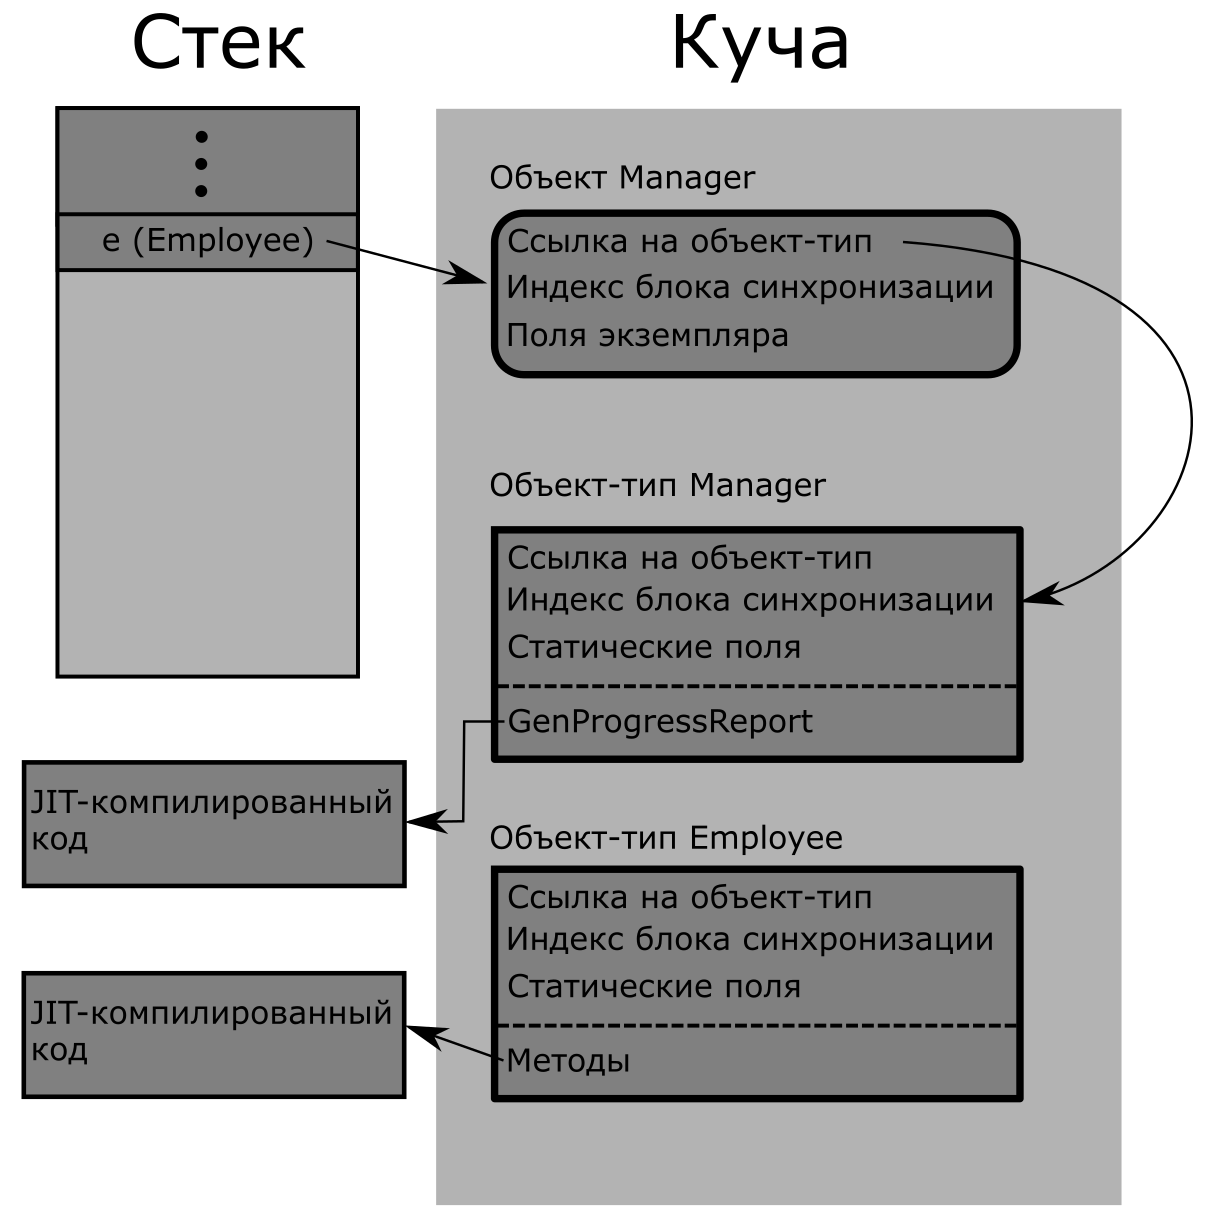
\includegraphics[width=0.5\textwidth]{objectInMemory.png}
\end{center}

На стеке вызовов находится ссылка на объект, сам объект лежит на куче. В участке памяти на куче назодится ссылка на объект-тип (она есть у всех объектов, даже у объектов-типов, такие дела), индекс блока синхронизации (штука, нужная для многопоточного программирования, это просто число) и значения полей объекта. В объекте-типе помимо всего вышеперечисленного лежат ещё статические поля класса, к которому принадлежит наш объект, и ссылки на скомпилированный код всех его методов.

\end{document}
